\documentclass{article}

\usepackage{graphicx}
\usepackage[margin=1in]{geometry}
\usepackage{booktabs}
\usepackage{float}
\usepackage{amsmath}
\usepackage[hidelinks]{hyperref}

\begin{document}

\title{QMC Kernel-Bank Approach Report}
\author{}
\date{4 March 2026}
\maketitle

\section*{Approach}
\subsection*{1. QMC-configured kernel pipeline}
The QMC setup configures the kernel bank with:
\begin{itemize}
    \item Sampling method: \texttt{qmc} (Sobol low-discrepancy sampling),
    \item Seed: 42,
    \item Scrambling: enabled.
\end{itemize}

Core pipeline settings used in the compared runs:
\begin{itemize}
    \item Patch setup: patch size $128$, inside/outside sampling $40/10$ per image.
    \item Kernel bank: 9 families, 500 kernels/family ($4500$ total), kernel size $31$.
    \item Selection: MMR, \texttt{topM}=3250, selected \(K=90\) kernels.
    \item Classifier: logistic, epochs $=60$, batch size $=64$, learning rate $=5\times10^{-4}$.
    \item Composite stage: 8 composite kernels built from 1250 selected-source kernels (uniform weights, L1 normalization).
\end{itemize}

\section*{Run Summary}
Method comparison is performed between two runs with the same MMR/composite settings:
\begin{itemize}
    \item \textbf{Random sampling baseline}.
    \item \textbf{QMC sampling method}.
    \item Both runs use: 4500 kernels, MMR selection with \(K=90\), and 8 composite kernels.
\end{itemize}

\section*{Results}
\subsection*{2. Test-set method comparison}
\begin{center}
\begin{tabular}{lccc}
\toprule
Evaluation (Test only) & Random sampling & QMC sampling & $\Delta$(QMC $-$ Random) \\
\midrule
Base model AUC & 0.919535 & \textbf{0.938699} & +0.019164 \\
Base model ACC & 0.864571 & \textbf{0.886631} & +0.022060 \\
Composite model AUC & 0.885451 & \textbf{0.893402} & +0.007952 \\
Composite model ACC & 0.806286 & \textbf{0.817647} & +0.011361 \\
\bottomrule
\end{tabular}
\end{center}

\textbf{Interpretation:}
\begin{itemize}
    \item On the available test results, QMC improves both AUC and ACC for the base and composite models relative to random sampling.
    \item The strongest gain appears in the base model AUC (+0.0192 absolute).
\end{itemize}

\section*{Classifier and Kernel Visualizations}
\begin{figure}[H]
    \centering
    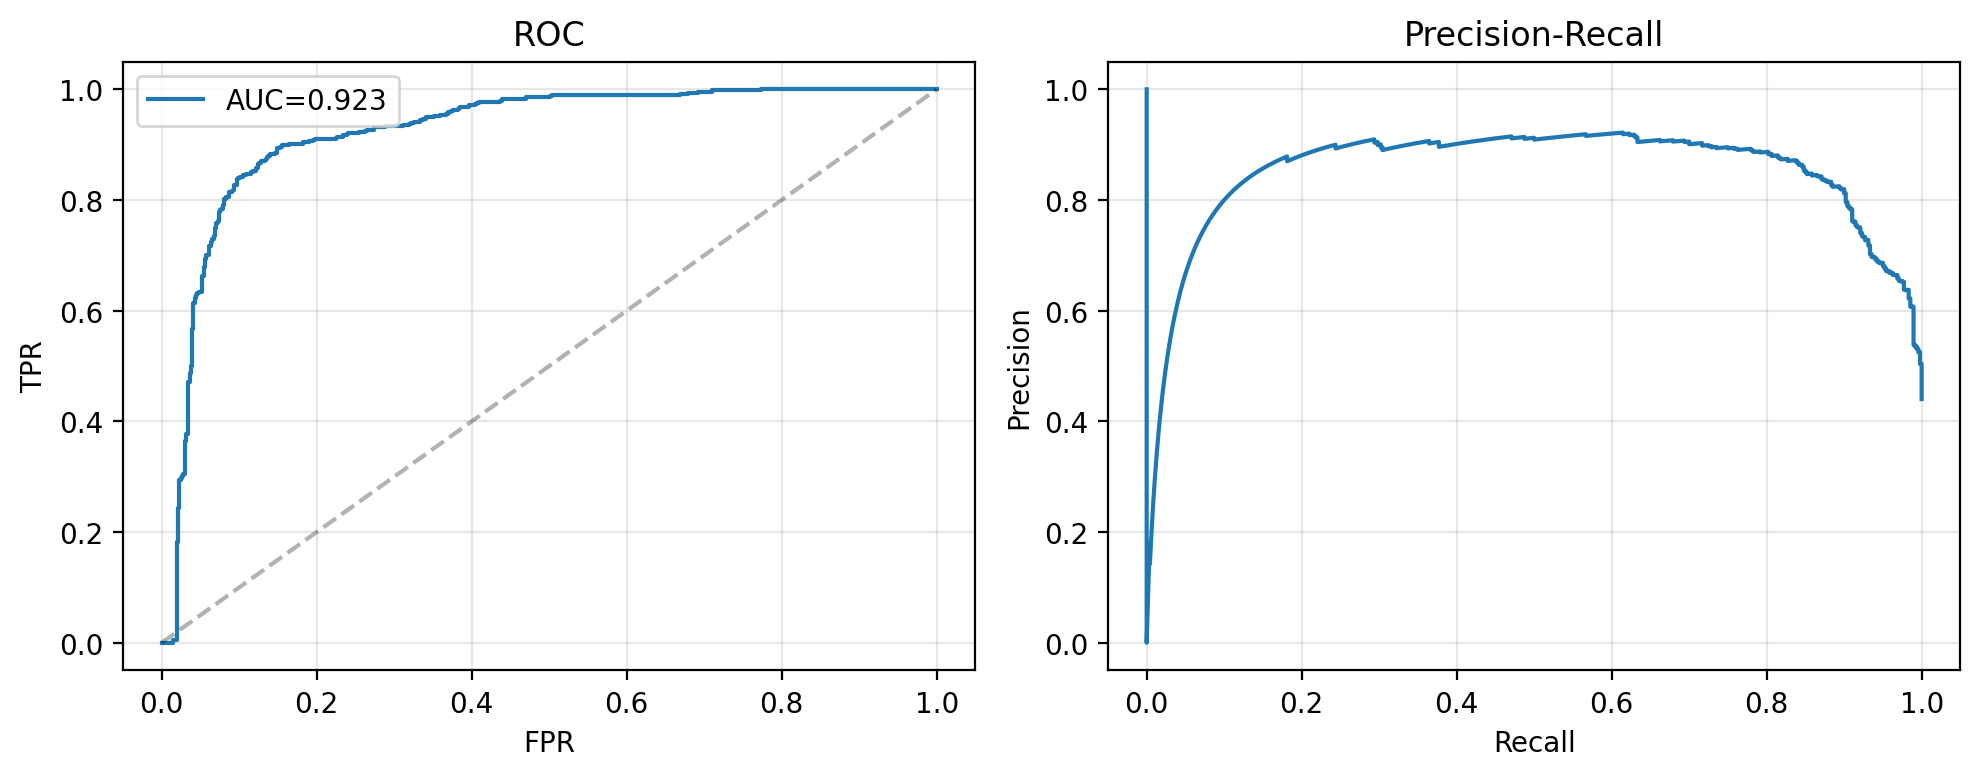
\includegraphics[width=0.49\linewidth]{../results/exp_024_8compositing/clf_roc_pr.png}
    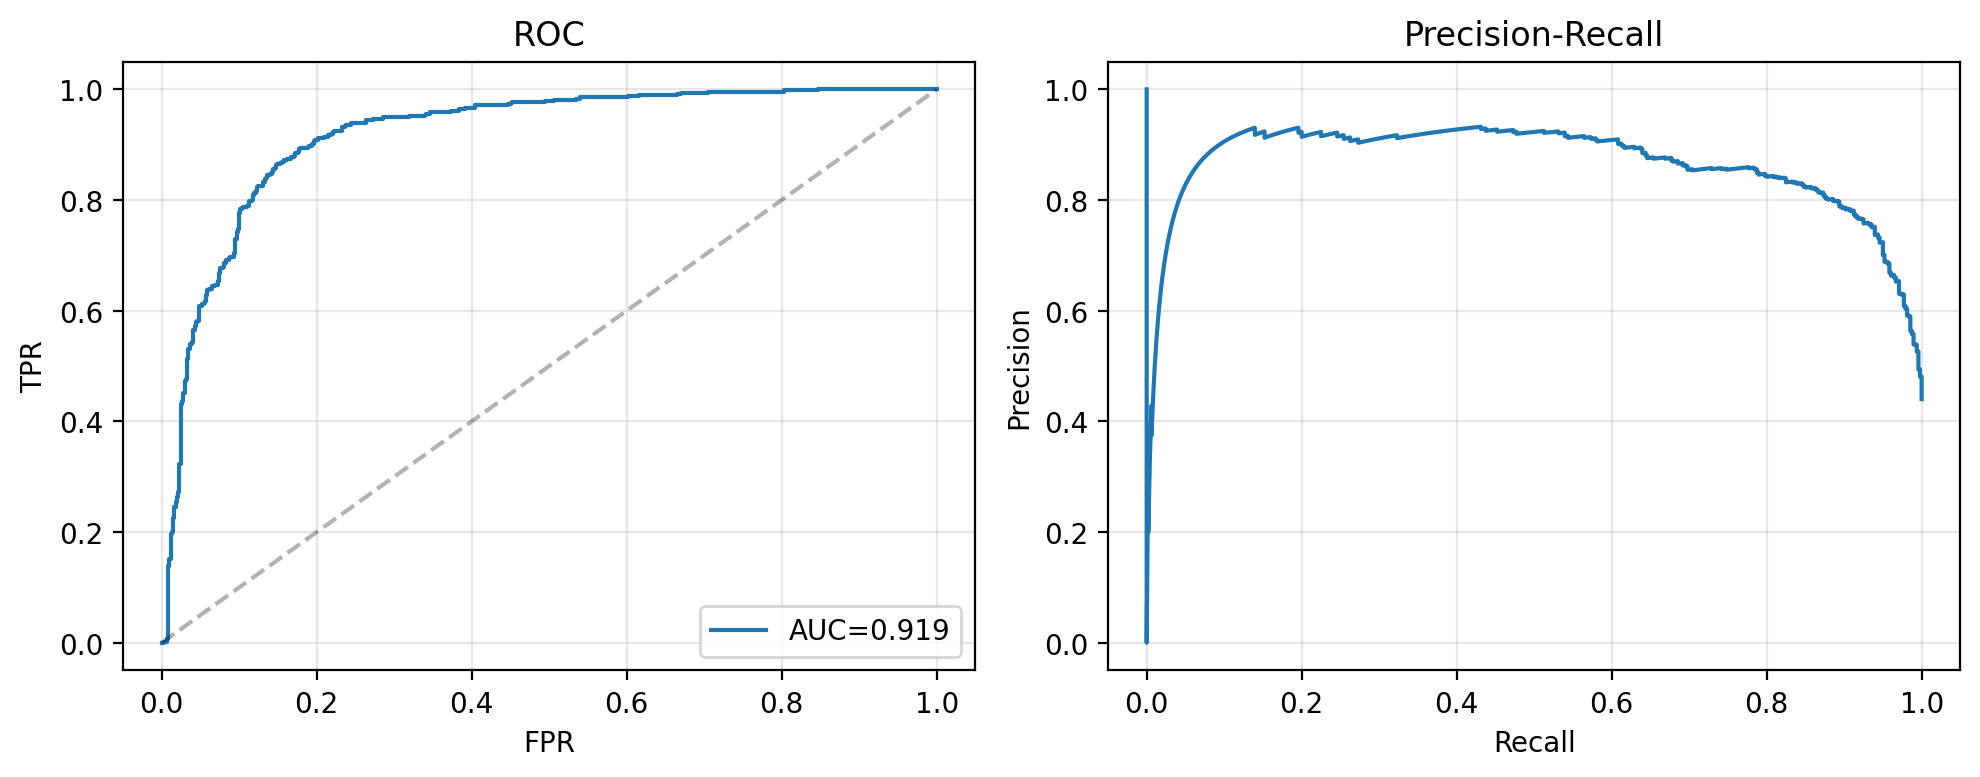
\includegraphics[width=0.49\linewidth]{../results/exp_024_8compositing/composite_roc_pr.png}
    \caption{Left: ROC/PR for selected-kernel base classifier. Right: ROC/PR for composite classifier.}
\end{figure}

\begin{figure}[H]
    \centering
    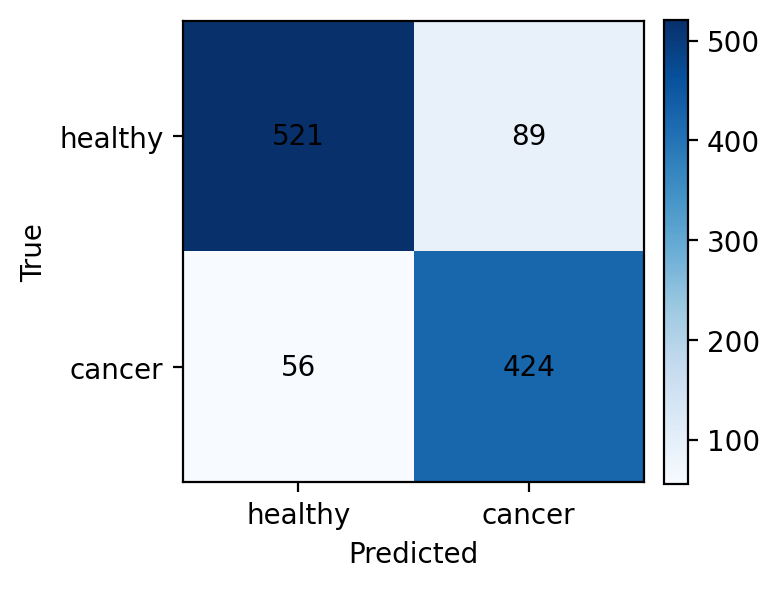
\includegraphics[width=0.49\linewidth]{../results/exp_024_8compositing/confusion.png}
    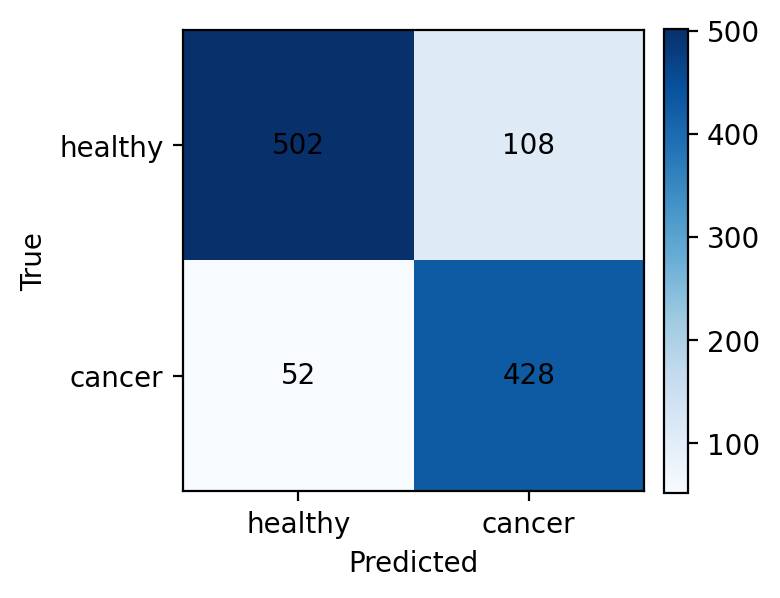
\includegraphics[width=0.49\linewidth]{../results/exp_024_8compositing/confusion_composite.png}
    \caption{Confusion matrices for base (left) and composite (right) classifiers.}
\end{figure}

\section*{Full-Image Inference + Heatmaps}
The notebook generates heatmaps for \texttt{IMG015}, \texttt{IMG044}, \texttt{IMG059}, and \texttt{IMG330} using the composite model and sliding-window aggregation.

\begin{figure}[H]
    \centering
    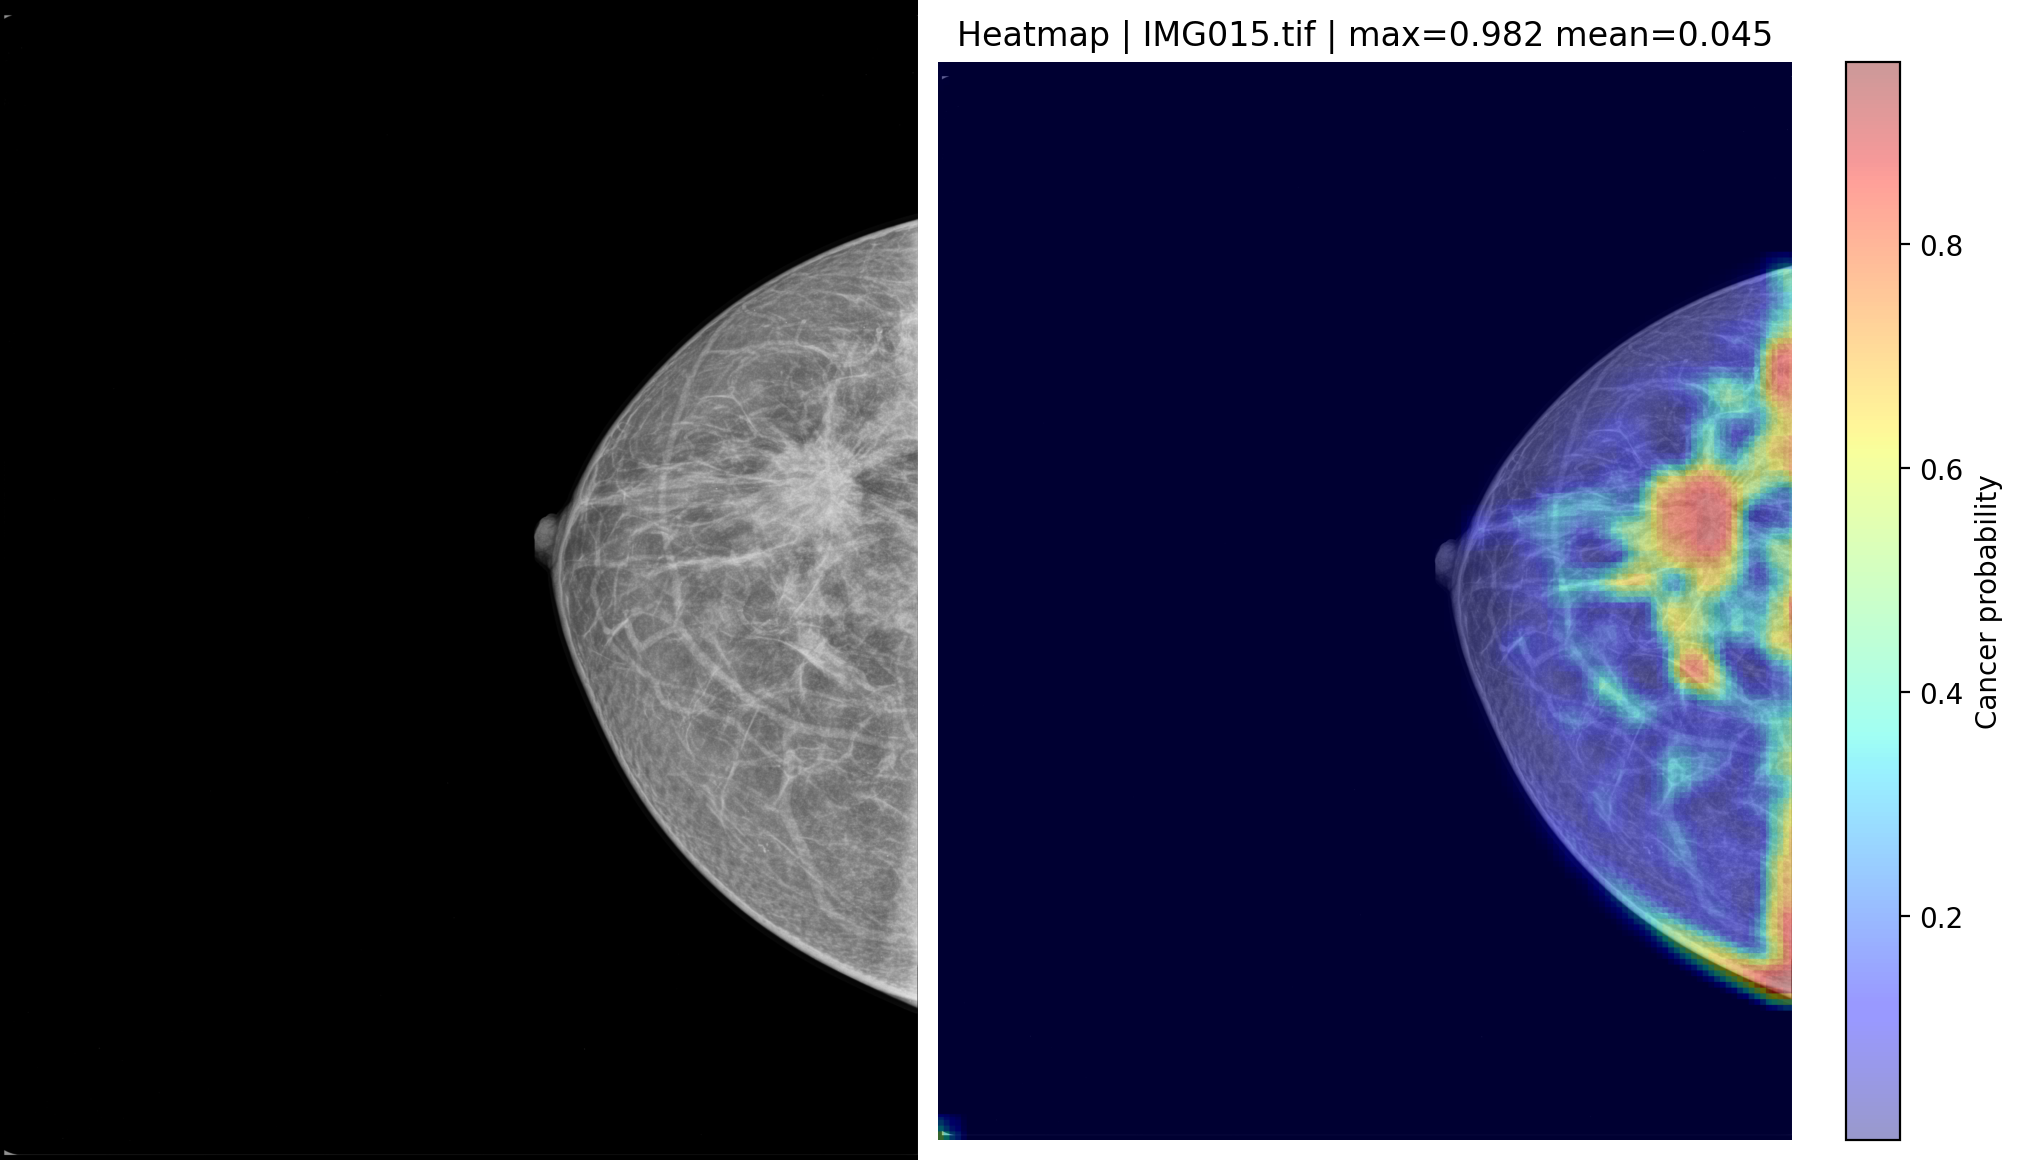
\includegraphics[width=0.49\linewidth]{../results/exp_024_8compositing/heatmaps_pairs/IMG015_pair.png}
    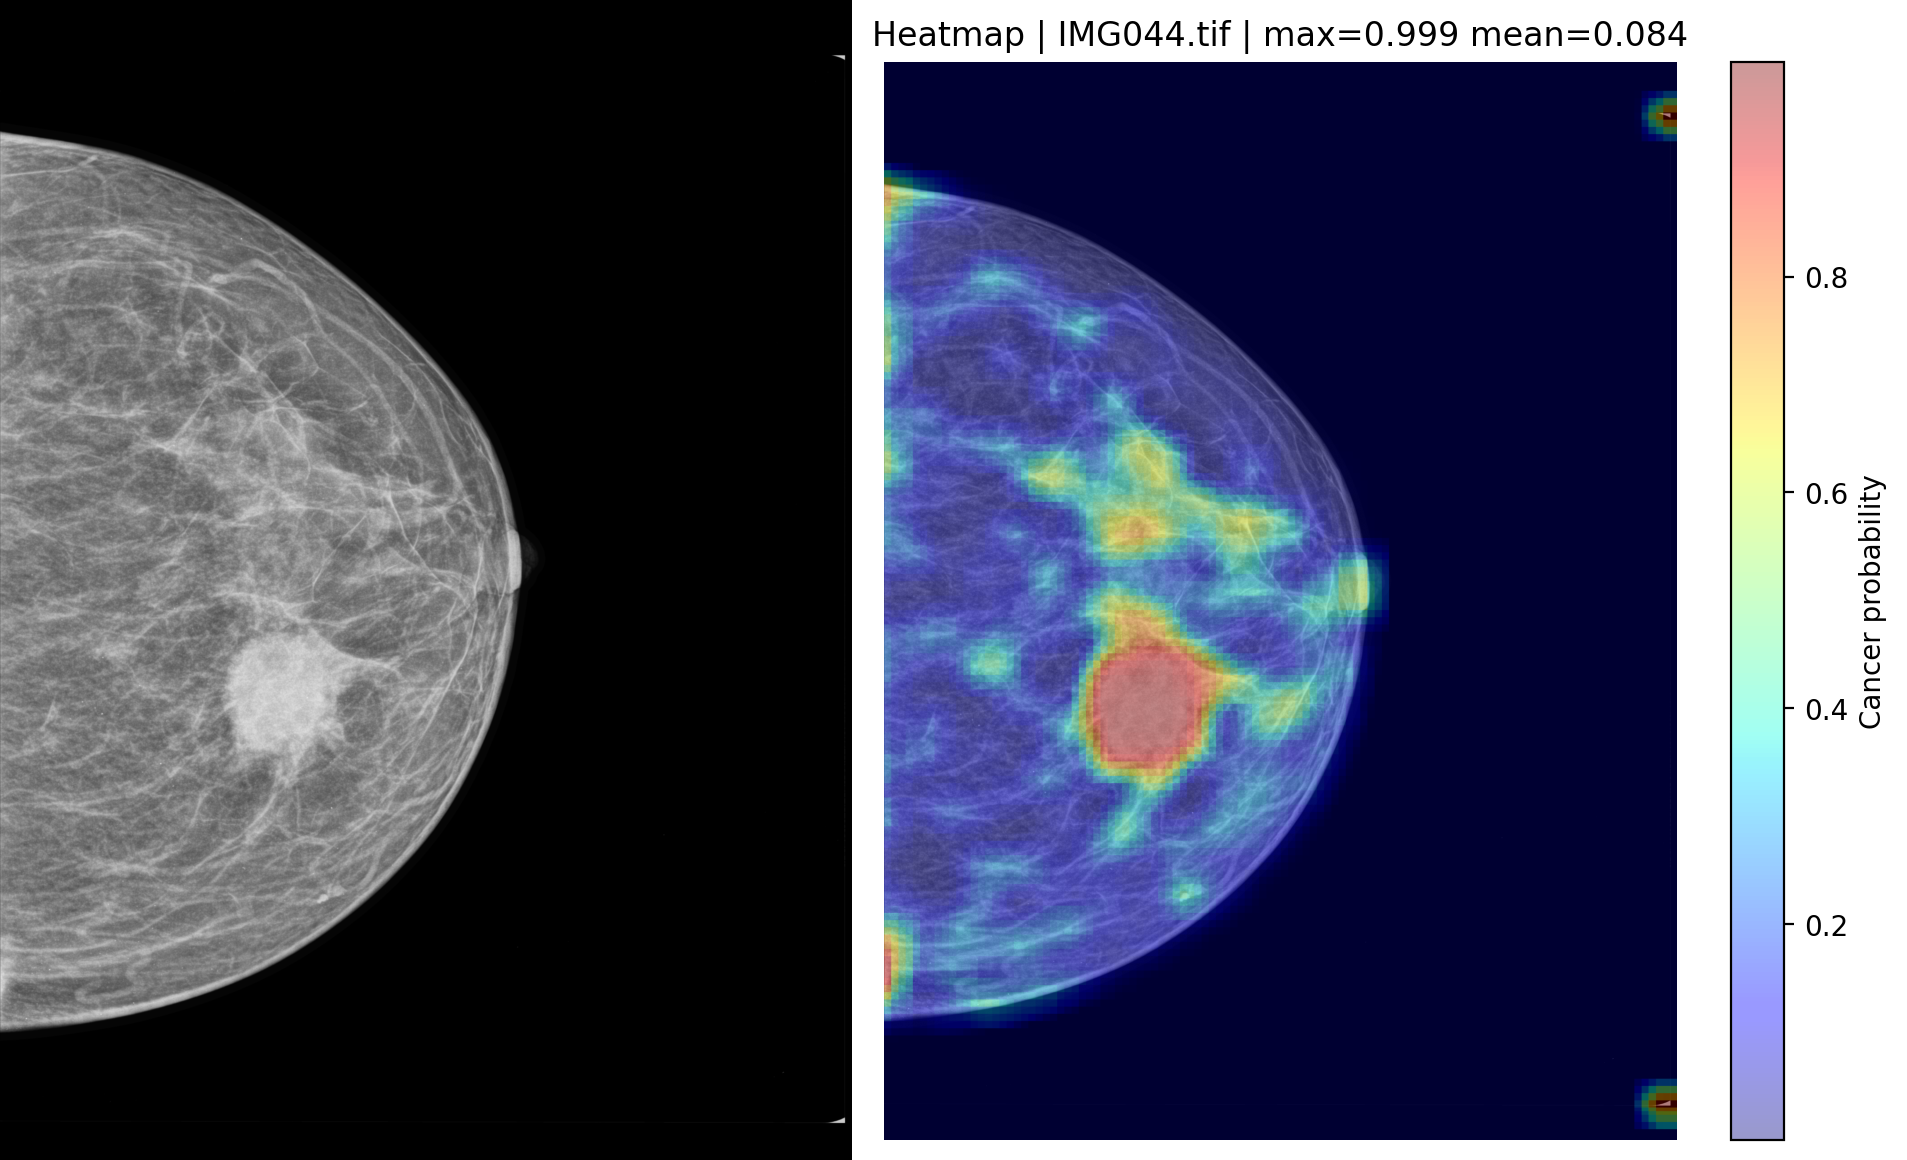
\includegraphics[width=0.49\linewidth]{../results/exp_024_8compositing/heatmaps_pairs/IMG044_pair.png}
    \caption{Composite-kernel heatmap pairs (set 1). Left image in each pair is original, right is overlay heatmap.}
\end{figure}

\begin{figure}[H]
    \centering
    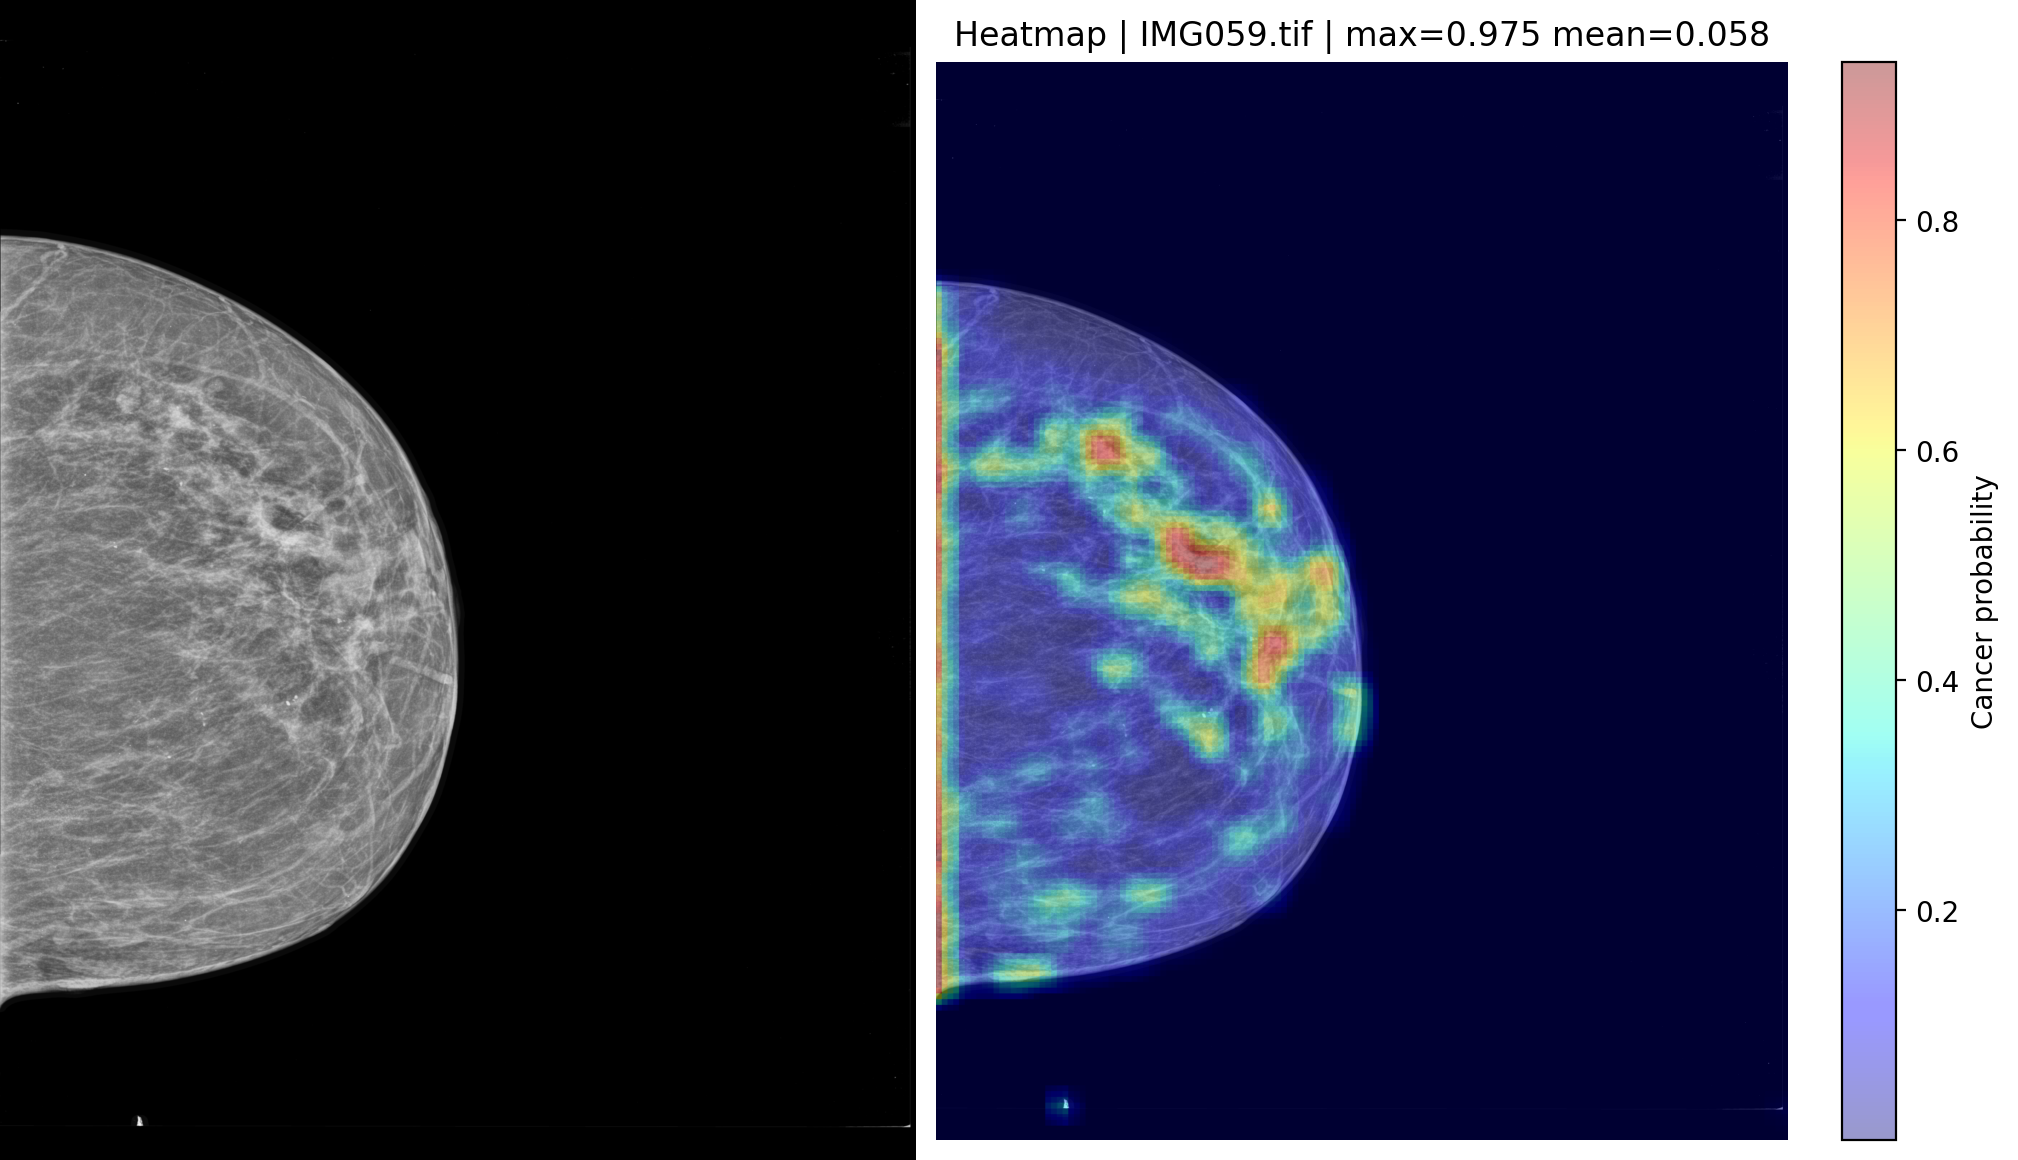
\includegraphics[width=0.49\linewidth]{../results/exp_024_8compositing/heatmaps_pairs/IMG059_pair.png}
    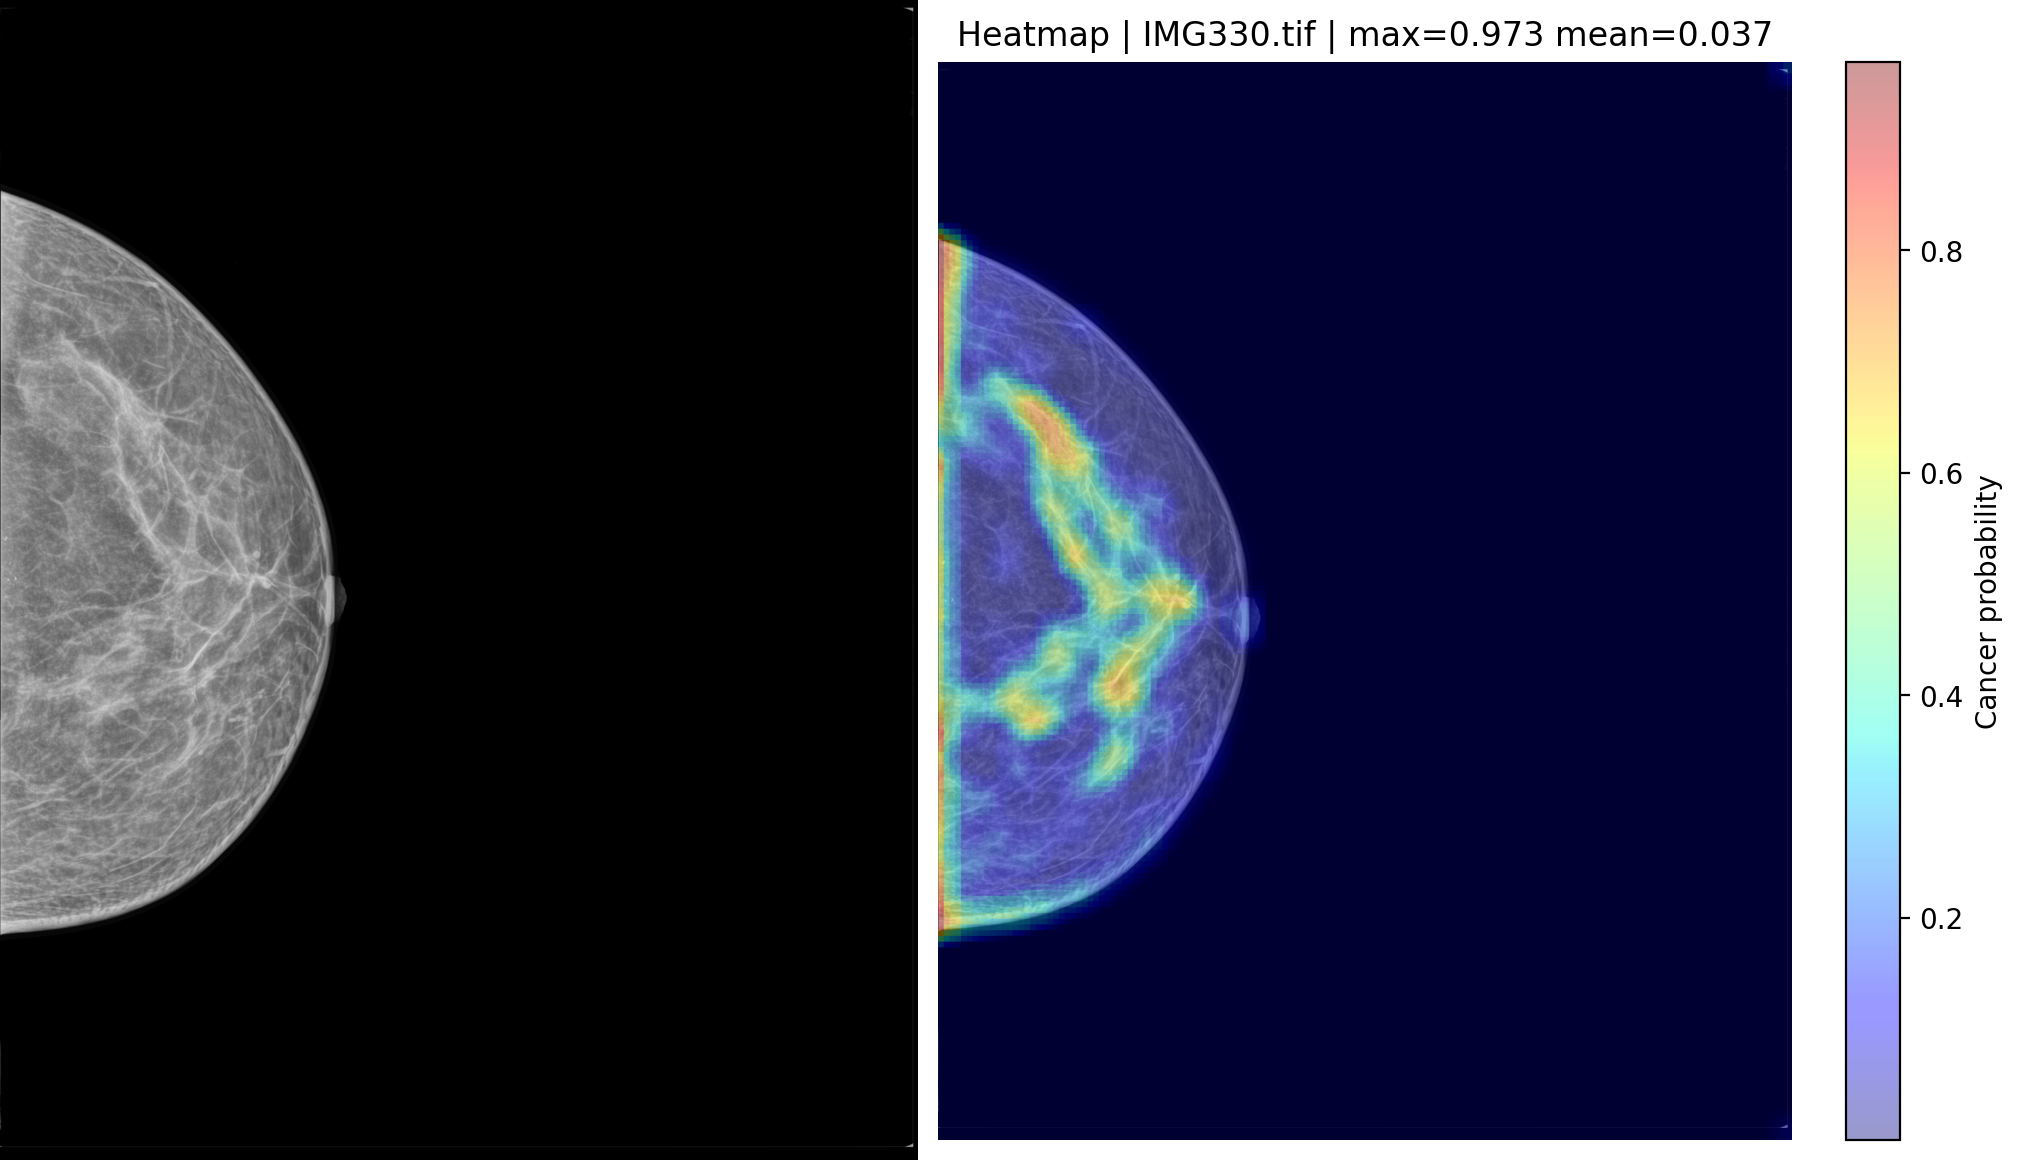
\includegraphics[width=0.49\linewidth]{../results/exp_024_8compositing/heatmaps_pairs/IMG330_pair.png}
    \caption{Composite-kernel heatmap pairs (set 2).}
\end{figure}

\section*{Findings}
\begin{itemize}
    \item QMC sampling outperforms random sampling on all reported test metrics in this comparison.
    \item The gain is largest for the base classifier AUC, and positive but smaller for the composite classifier.
\end{itemize}

\section*{Next Steps}
\begin{itemize}
    \item Combine QMC and composite-kernel training by training composite kernels on data with \(f_i\) from 1 to 10.
\end{itemize}

\section*{Conclusion}
In this report comparison, QMC is better than random sampling on all reported test metrics (base and composite, AUC and ACC). The evidence supports QMC as the preferred sampling method for this kernel-bank pipeline.

\end{document}
